\chapter{Related Work}

This chapter outlines the major studies in ontology matching methodologies and specifically targets the field of instance matching, by providing a high-level classification with respect to their main characteristics. Based on these methods, the structures of the most recent and impactful matching systems are introduced along with their latest evaluation results.


\section{Classification of Techniques}

Many approaches have been proposed for the classification of ontology matching techniques. For example, one way is to look at the input, process and output dimensions of the algorithms \cite{euzenat2013d}. Characteristics such as the representation models accepted as input, the type of context used, and the cardinality of output alignments are taken into account. Another way is to distinguish between local methods that directly target the properties of the entities, such as string comparison, and globals methods that investigate into the structures that hold the entities together, such as graph segments. The most accepted classification method was proposed by Jérôme Euzenat and Pavel Shvaiko, which considers the different sources and interpretations of the input information, and further classify them with respect to how they are being processed \cite{euzenat2013d}. Other classification methods from different inspirations exist \cite{DBLP:conf/swb/Ehrig2007,DBLP:conf/icde/MadhavanBDH05}, but the ideas are generally similar.
\\\\
Based on the fundamental differences identified in the above mentioned approaches, this section describes a classification method focusing on the algorithmic characteristics of the local methodologies used for ontology matching. The proposed classification is shown in Figure \ref{fig:techniques}.

\begin{figure}[ht]
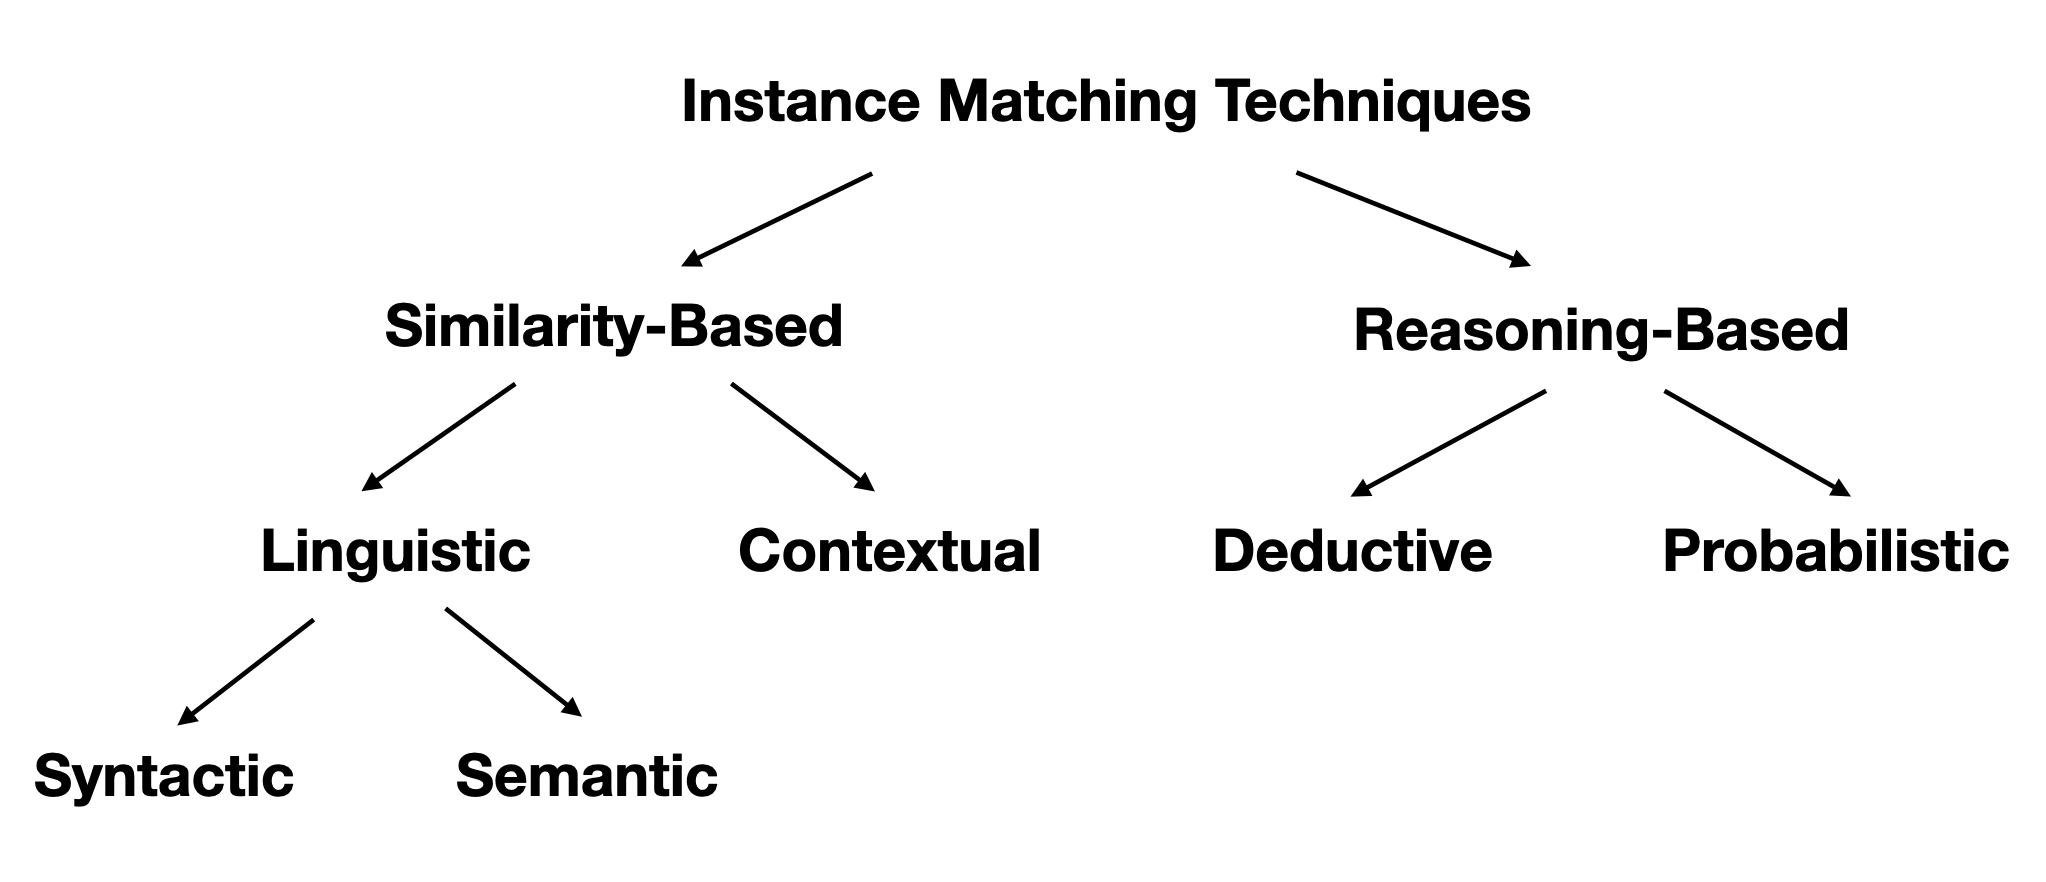
\includegraphics[width=\textwidth]{img/ontology_matching_classification.png}
\caption{Classification of Ontology Matching Techniques}
\label{fig:techniques}
\end{figure}

\subsection{Similarity-based}

Similarity-based techniques try to perform a quantitative measurement on the degree of similarity of two entities. Generally speaking, entities are concrete ontological components such as classes, datatypes, properties, and named individuals, and while the main focus is in the context of instance matching, all of them should be considered to facilitate the design of the whole structure. Linguistic similarity and contextual similarity are the two most-used criteria for the measurement \cite{DBLP:conf/ic3k/Nguyen015}.

\subsubsection{Linguistic Similarity}

The linguistic components of an instance are the characteristics related to its string representation. For similarity measurements of strings, syntactic analysis and semantic analysis are the two main approaches.
\\\\
% Syntactic.
The syntactical components of an instance can be the string structure of its name and description, its type constraints, the list of properties it possesses, and so on. Syntactic techniques take advantage of these string structures to discover different kinds and levels of similarities. For example, measures like Edit Distance, Smith-Waterman Distance, and Jaro Distance are based on characters \cite{DBLP:journals/corr/SekerAAM14,DBLP:journals/algorithmica/FaroMP20}, while measures like Cosine Similarity and Q-Gram Distance are based on tokens \cite{DBLP:conf/wea/KobayashiHYS20}. Different weights can be introduced according to the occurrence frequency of the values, so that matches of rare values can receive higher confidence \cite{DBLP:conf/dsit/WangN20}. Further more, phonetic similarities can be discovered with techniques like Soundex \cite{DBLP:journals/corr/BhattiWIHS14} and Metaphone \cite{DBLP:conf/cicling/JordaoR12}, even though their string representations are very different.
\\\\
% Semantic.
Semantic approaches, in contrast, seek to analyse the actual meaning of the entities to be matched, either by informal methods such as looking up dictionaries or thesauri and reading the annotations \cite{DBLP:journals/corr/abs-0907-2209,DBLP:conf/ifip12/LinS08,DBLP:conf/esws/Vennesland15}, or formal methods such as deriving the meaning from semantic definition in other ontologies. Techniques based on this approach first expand the meanings of entities to be matched with synonyms and hyponyms, then evaluate the intersection of their meanings to perform similarity calculations \cite{DBLP:conf/ieaaie/AssiMD19}.

\subsubsection{Contextual Similarity}

Context-based techniques try to match the instances by considering not only their personal attributes, but also how they are defined in their respective ``contexts'', such as object properties and semantic relations with other instances \cite{DBLP:journals/jucs/LinSX12}. The context of an entity can typically be represented as a graph, where entities are denoted by nodes, and properties and semantic relations are denoted by edges. Graph matching algorithms can then be applied to evaluate the topological similarity between the context graphs, therefore determine the similarity between those instances \cite{DBLP:conf/kdd/JehW02}.

\subsection{Reasoning-based}

A fundamental difference between reasoning-based techniques and similarity-based ones is that, in order that reasonings can start, the existence of an initial set of alignments is required as a foundation \cite{DBLP:conf/esws/Meilicke09}. These alignments can be semantic relations already existing between the two ontologies, or manually established by domain experts, or acquired automatically through some similarity-based techniques. Based on these initial alignments, implications of new alignments can be derived by performing various kinds of reasoning tasks. The process goes on iteratively based on the new alignments discovered in the previous iterations, until a time limit or a fixed number of iterations is reached, or no new alignments can be discovered \cite{DBLP:journals/logcom/MeilickeST09}.

\subsubsection{Deductive Reasoning}

Most of the reasoning techniques are considered deductive, as they typically use implication models in the derivation of new candidate alignments. The propositional satisfiability (SAT) model \cite{DBLP:journals/ai/PhamTS08}, for example, treats a candidate alignment between two instances as a propositional formula or implication, whose satisfiability is checked with SAT solvers to determine the correctness of the candidate alignment. Another widely adopted deductive approach is based on the description logic model, in which case existing alignments are used together with axioms in the respective ontology such as subsumptions, to exploit and infer new alignments to enrich the initial set \cite{DBLP:phd/ethos/Reul12}.

\subsubsection{Probabilistic Reasoning}

Probabilistic reasoning approaches, on the other hand, try to compute the probability that two entities are identical or similar, by checking whether they have similar hierarchical structure or semantic relations \cite{DBLP:conf/esws/CastanoFLNM08}. Most of them utilise heuristic algorithms \cite{DBLP:conf/jist/NguyenI15}, machine learning techniques or Bayesian networks \cite{DBLP:conf/semweb/SvabS06} for the calculation and propagation of joint probabilities. The interest in techniques that adopt machine learning have been increasing in recent years, however the difficulty in finding a good training dataset is still challenging. Other related techniques based on data analysis and statistical techniques include fuzzy ontologies \cite{DBLP:conf/semweb/TodorovHG13}.


\section{Matching Systems}

A number of matching systems have been proposed in this area, some for general purposes and the other target specific use cases. The list below selects the ones that are most impactful and have distinctive characteristics and gives a brief description of the methodologies they employ \cite{euzenat2013d}.

\begin{spacing}{1.2}
\begin{enumerate}
	\item H-Match: Computes linguistic and contextual similarities and then combine them with weighting schemas to give the final measure of semantic affinity. Common thesauri are used and extended to consider taxonomical or mereological relations.
	\item COMA++: A schema matching tool that utilises string-based techniques, auxiliary thesauri and parallel composition of matchers. Semantically it supports alignment reuse, and structurally it promotes Directed Acyclic Graph (DAG) matching.
	\item MapOnto: A semi-automated system that constructs complex mapping formulas in Horn clauses. Simple external alignments are taken as part of the input, and structural comparison between the graphical representation of input ontologies are performed.
	\item CtxMatch: Besides the semantic approaches based on strings and WordNet, it exploits description logic reasoners such as Pellet \cite{DBLP:journals/ws/SirinPGKK07} and FaCT \cite{DBLP:conf/cade/TsarkovH06}.
	\item S-Match: Semantic matching is performed based on strings and languages. Entity relations are then translated into propositional formulas using the WordNet dictionary, and resolved with SAT solvers.
	\item Lily: Combines string-based techniques such as Levenshtein Distance and structure-based techniques such as variations of Similarity Flooding, to handle large ontologies.
	\item OLA: Compiles the input ontologies into graph structures, then computes string-based, language-based and structure-based similarities. An iterative fixed point algorithm is then performed until no improvements can be discovered.
	\item RiMOM: Uses Bayesian decision theory to automatically discover complex alignments. Taxonomic structure similarities are heuristically discovered and then propagated.
	\item LogMap: Performs lexical indexing using string-based methods and with the help of WordNet. The tree structures of indices are compared, and the matches are repaired using the Dowling-Gallier algorithm based on propositional Horn satisfiability.
	\item PARIS: A probabilistic system that aligns relations, instances and schemas via iterative fixed point computation.
\end{enumerate}
\end{spacing}

It can be discovered that most of the matching systems are schema-based, and tend to focus on specific application domains. Only few of them target the general problem, such as COMA++ and S-Match. Another concern is that most of them handle tree structures while only COMA++ and OLA handle graphs. Further more, only few of them can discover complex correspondences other than the simple one-to-one. And Finally, most of them lack a graphical user interface \cite{euzenat2013d}.
\\\\
The Ontology Alignment Evaluation Initiative (OAEI)\footnote{\url{http://oaei.ontologymatching.org/}} is a coordinated international initiative to assess strengths and weaknesses of alignment or matching systems, and to compare performance of techniques. It has been organising ontology matching workshops since 2004. Tables \ref{tab:SPIMBENCH_SANDBOX_2020}, \ref{tab:SPIMBENCH_MAINBOX_2020}, \ref{tab:Knowledge_Graph_2020_Overview}, \ref{tab:Knowledge_Graph_2020_Instance_Results} shows the most recent results in 2020 for the SPIMBENCH and Knowledge Graph tracks for the matching systems participated\footnote{\url{https://project-hobbit.eu/challenges/om2020/}}. The reason of considering only these results is that those evaluation tracks focus specifically on instance matching. It can be seen that Lily has achieved excellent precision and recall rate within acceptable time frame, while AML and ATBox outperforms the others in instance matching for Knowledge Graph.

\begin{table}[ht!]
\resizebox{\textwidth}{!}{%
\begin{tabular}{|l|l|l|l|l|l|}
\hline
System          & LogMap-HOBBIT & AgreementMakerLight-Hobbit & Lily\_HOBBIT-2.2 & FTRLIM      & REMiner-1.5 \\ \hline
Fmeasure        & 0.841328413   & 0.864516129                & 0.991708126      & 0.921417565 & 0.998324958 \\ \hline
Precision       & 0.938271605   & 0.834890966                & 0.983552632      & 0.854285714 & 1           \\ \hline
Recall          & 0.762541806   & 0.89632107                 & 1                & 1           & 0.996655518 \\ \hline
timePerformance & 7483          & 6446                       & 2050             & 1525        & 7284        \\ \hline
\end{tabular}%
}
\caption{SPIMBENCH SANDBOX 2020}
\label{tab:SPIMBENCH_SANDBOX_2020}
\end{table}

\begin{table}[ht!]
\resizebox{\textwidth}{!}{%
\begin{tabular}{|l|l|l|l|l|l|}
\hline
System          & LogMap-HOBBIT & AgreementMakerLight-Hobbit & Lily\_HOBBIT-2.2 & FTRLIM      & REMiner-1.5 \\ \hline
Fmeasure        & 0.785635764   & 0.860457622                & 0.995388669      & 0.921478766 & 0.997681351 \\ \hline
Precision       & 0.880131363   & 0.838567839                & 0.990819672      & 0.85584563  & 0.99867374  \\ \hline
Recall          & 0.709463931   & 0.883520847                & 1                & 0.99801456  & 0.996690933 \\ \hline
timePerformance & 26782         & 38772                      & 3899             & 2247        & 33966       \\ \hline
\end{tabular}%
}
\caption{SPIMBENCH MAINBOX 2020}
\label{tab:SPIMBENCH_MAINBOX_2020}
\end{table}

\begin{table}[ht!]
\resizebox{\textwidth}{!}{%
\begin{tabular}{|l|l|l|l|l|l|l|l|l|l|l|l|l|l|l|l|l|l|l|}
\hline
\multicolumn{1}{|c|}{\textbf{}}       & \multicolumn{1}{c|}{\textbf{}}     & \multicolumn{4}{c|}{\textbf{class}}                                                                                                                       & \multicolumn{4}{c|}{\textbf{property}}                                                                                                             & \multicolumn{4}{c|}{\textbf{instance}}                                                                                                             & \multicolumn{4}{c|}{\textbf{overall}}                                                                                                              &                                    \\ \hline
\multicolumn{1}{|c|}{\textbf{System}} & \multicolumn{1}{c|}{\textbf{Time}} & \multicolumn{1}{c|}{\textbf{\#testcases}} & \multicolumn{1}{c|}{\textbf{Size}} & \multicolumn{1}{c|}{\textbf{Prec.}} & \multicolumn{1}{c|}{\textbf{F-m.}} & \multicolumn{1}{c|}{\textbf{Rec.}} & \multicolumn{1}{c|}{\textbf{Size}} & \multicolumn{1}{c|}{\textbf{Prec.}} & \multicolumn{1}{c|}{\textbf{F-m.}} & \multicolumn{1}{c|}{\textbf{Rec.}} & \multicolumn{1}{c|}{\textbf{Size}} & \multicolumn{1}{c|}{\textbf{Prec.}} & \multicolumn{1}{c|}{\textbf{F-m.}} & \multicolumn{1}{c|}{\textbf{Rec.}} & \multicolumn{1}{c|}{\textbf{Size}} & \multicolumn{1}{c|}{\textbf{Prec.}} & \multicolumn{1}{c|}{\textbf{F-m.}} & \multicolumn{1}{c|}{\textbf{Rec.}} \\ \hline
ALOD2Vec                              & 0:13:24                            & 5                                         & 20.0                               & 1.00 (1.00)                         & 0.80 (0.80)                        & 0.67 (0.67)                        & 76.8                               & 0.94 (0.94)                         & 0.95 (0.95)                        & 0.97 (0.97)                        & 4893.8                             & 0.91 (0.91)                         & 0.87 (0.87)                        & 0.83 (0.83)                        & 4990.6                             & 0.91 (0.91)                         & 0.87 (0.87)                        & 0.83 (0.83)                        \\ \hline
AML                                   & 0:50:55                            & 5                                         & 23.6                               & 0.98 (0.98)                         & 0.89 (0.89)                        & 0.81 (0.81)                        & 48.4                               & 0.92 (0.92)                         & 0.70 (0.70)                        & 0.57 (0.57)                        & 6802.8                             & 0.90 (0.90)                         & 0.85 (0.85)                        & 0.80 (0.80)                        & 6874.8                             & 0.90 (0.90)                         & 0.85 (0.85)                        & 0.80 (0.80)                        \\ \hline
ATBox                                 & 0:16:22                            & 5                                         & 25.6                               & 0.97 (0.97)                         & 0.87 (0.87)                        & 0.79 (0.79)                        & 78.8                               & 0.97 (0.97)                         & 0.96 (0.96)                        & 0.95 (0.95)                        & 4858.8                             & 0.89 (0.89)                         & 0.84 (0.84)                        & 0.80 (0.80)                        & 4963.2                             & 0.89 (0.89)                         & 0.85 (0.85)                        & 0.81 (0.81)                        \\ \hline
baselineAltLabel                      & 0:10:57                            & 5                                         & 16.4                               & 1.00 (1.00)                         & 0.74 (0.74)                        & 0.59 (0.59)                        & 47.8                               & 0.99 (0.99)                         & 0.79 (0.79)                        & 0.66 (0.66)                        & 4674.8                             & 0.89 (0.89)                         & 0.84 (0.84)                        & 0.80 (0.80)                        & 4739.0                             & 0.89 (0.89)                         & 0.84 (0.84)                        & 0.80 (0.80)                        \\ \hline
baselineLabel                         & 0:10:44                            & 5                                         & 16.4                               & 1.00 (1.00)                         & 0.74 (0.74)                        & 0.59 (0.59)                        & 47.8                               & 0.99 (0.99)                         & 0.79 (0.79)                        & 0.66 (0.66)                        & 3641.8                             & 0.95 (0.95)                         & 0.81 (0.81)                        & 0.71 (0.71)                        & 3706.0                             & 0.95 (0.95)                         & 0.81 (0.81)                        & 0.71 (0.71)                        \\ \hline
DESKMatcher                           & 0:13:54                            & 5                                         & 91.4                               & 0.76 (0.76)                         & 0.71 (0.71)                        & 0.66 (0.66)                        & 0.0                                & 0.00 (0.00)                         & 0.00 (0.00)                        & 0.00 (0.00)                        & 3820.6                             & 0.94 (0.94)                         & 0.82 (0.82)                        & 0.74 (0.74)                        & 3912.0                             & 0.93 (0.93)                         & 0.81 (0.81)                        & 0.72 (0.72)                        \\ \hline
LogMap                                & 2:55:14                            & 5                                         & 24.0                               & 0.95 (0.95)                         & 0.84 (0.84)                        & 0.76 (0.76)                        & 0.0                                & 0.00 (0.00)                         & 0.00 (0.00)                        & 0.00 (0.00)                        & 29190.4                            & 0.40 (0.40)                         & 0.54 (0.54)                        & 0.86 (0.86)                        & 29214.4                            & 0.40 (0.40)                         & 0.54 (0.54)                        & 0.84 (0.84)                        \\ \hline
LogMapBio                             & 4:35:29                            & 5                                         & 24.0                               & 0.95 (0.95)                         & 0.84 (0.84)                        & 0.76 (0.76)                        & 0.0                                & 0.00 (0.00)                         & 0.00 (0.00)                        & 0.00 (0.00)                        & 0.0                                & 0.00 (0.00)                         & 0.00 (0.00)                        & 0.00 (0.00)                        & 24.0                               & 0.95 (0.95)                         & 0.01 (0.01)                        & 0.00 (0.00)                        \\ \hline
LogMapIM                              & 2:49:34                            & 5                                         & 0.0                                & 0.00 (0.00)                         & 0.00 (0.00)                        & 0.00 (0.00)                        & 0.0                                & 0.00 (0.00)                         & 0.00 (0.00)                        & 0.00 (0.00)                        & 29190.4                            & 0.40 (0.40)                         & 0.54 (0.54)                        & 0.86 (0.86)                        & 29190.4                            & 0.40 (0.40)                         & 0.54 (0.54)                        & 0.84 (0.84)                        \\ \hline
LogMapKG                              & 2:47:51                            & 5                                         & 24.0                               & 0.95 (0.95)                         & 0.84 (0.84)                        & 0.76 (0.76)                        & 0.0                                & 0.00 (0.00)                         & 0.00 (0.00)                        & 0.00 (0.00)                        & 29190.4                            & 0.40 (0.40)                         & 0.54 (0.54)                        & 0.86 (0.86)                        & 29214.4                            & 0.40 (0.40)                         & 0.54 (0.54)                        & 0.84 (0.84)                        \\ \hline
LogMapLt                              & 0:07:19                            & 4                                         & 23.0                               & 0.80 (1.00)                         & 0.56 (0.70)                        & 0.43 (0.54)                        & 0.0                                & 0.00 (0.00)                         & 0.00 (0.00)                        & 0.00 (0.00)                        & 6653.8                             & 0.73 (0.91)                         & 0.67 (0.84)                        & 0.62 (0.78)                        & 6676.8                             & 0.73 (0.92)                         & 0.66 (0.83)                        & 0.61 (0.76)                        \\ \hline
Wiktionary                            & 0:30:12                            & 5                                         & 22.4                               & 1.00 (1.00)                         & 0.80 (0.80)                        & 0.67 (0.67)                        & 80.0                               & 0.94 (0.94)                         & 0.95 (0.95)                        & 0.97 (0.97)                        & 4893.8                             & 0.91 (0.91)                         & 0.87 (0.87)                        & 0.83 (0.83)                        & 4996.2                             & 0.91 (0.91)                         & 0.87 (0.87)                        & 0.83 (0.83)                        \\ \hline
\end{tabular}%
}
\caption{Knowledge Graph 2020 Overview}
\label{tab:Knowledge_Graph_2020_Overview}
\end{table}

\begin{table}[ht!]
\resizebox{\textwidth}{!}{%
\begin{tabular}{|l|l|l|l|l|l|l|l|l|l|l|l|l|l|l|l|l|l|l|l|l|}
\hline
\multicolumn{4}{|c|}{\textbf{marvelcinematicuniverse-marvel}}                                                                                   & \multicolumn{4}{c|}{\textbf{memoryalpha-memorybeta}}                                                                                               & \multicolumn{4}{c|}{\textbf{memoryalpha-stexpanded}}                                                                                               & \multicolumn{4}{c|}{\textbf{starwars-swg}}                                                                                                         & \multicolumn{4}{c|}{\textbf{starwars-swtor}}                                                                                                       &                                    \\ \hline
\multicolumn{1}{|c|}{\textbf{}} & \multicolumn{1}{c|}{\textbf{Size}} & \multicolumn{1}{c|}{\textbf{Prec.}} & \multicolumn{1}{c|}{\textbf{F-m.}} & \multicolumn{1}{c|}{\textbf{Rec.}} & \multicolumn{1}{c|}{\textbf{Size}} & \multicolumn{1}{c|}{\textbf{Prec.}} & \multicolumn{1}{c|}{\textbf{F-m.}} & \multicolumn{1}{c|}{\textbf{Rec.}} & \multicolumn{1}{c|}{\textbf{Size}} & \multicolumn{1}{c|}{\textbf{Prec.}} & \multicolumn{1}{c|}{\textbf{F-m.}} & \multicolumn{1}{c|}{\textbf{Rec.}} & \multicolumn{1}{c|}{\textbf{Size}} & \multicolumn{1}{c|}{\textbf{Prec.}} & \multicolumn{1}{c|}{\textbf{F-m.}} & \multicolumn{1}{c|}{\textbf{Rec.}} & \multicolumn{1}{c|}{\textbf{Size}} & \multicolumn{1}{c|}{\textbf{Prec.}} & \multicolumn{1}{c|}{\textbf{F-m.}} & \multicolumn{1}{c|}{\textbf{Rec.}} \\ \hline
ALOD2Vec                        & 3065                               & 0.86                                & 0.76                               & 0.68                               & 13325                              & 0.92                                & 0.91                               & 0.90                               & 3285                               & 0.92                                & 0.93                               & 0.93                               & 2118                               & 0.92                                & 0.82                               & 0.75                               & 2676                               & 0.92                                & 0.92                               & 0.91                               \\ \hline
AML                             & 4670                               & 0.85                                & 0.68                               & 0.56                               & 18319                              & 0.91                                & 0.89                               & 0.87                               & 3699                               & 0.93                                & 0.93                               & 0.93                               & 3491                               & 0.90                                & 0.81                               & 0.75                               & 3835                               & 0.93                                & 0.92                               & 0.90                               \\ \hline
ATBox                           & 3483                               & 0.66                                & 0.58                               & 0.52                               & 12860                              & 0.96                                & 0.93                               & 0.91                               & 3162                               & 0.96                                & 0.94                               & 0.92                               & 2170                               & 0.93                                & 0.83                               & 0.76                               & 2619                               & 0.94                                & 0.92                               & 0.91                               \\ \hline
baselineAltLabel                & 2559                               & 0.86                                & 0.76                               & 0.68                               & 13454                              & 0.88                                & 0.89                               & 0.89                               & 3165                               & 0.88                                & 0.90                               & 0.93                               & 1661                               & 0.92                                & 0.74                               & 0.62                               & 2535                               & 0.92                                & 0.91                               & 0.90                               \\ \hline
baselineLabel                   & 1864                               & 0.90                                & 0.69                               & 0.56                               & 10492                              & 0.95                                & 0.85                               & 0.77                               & 2517                               & 0.98                                & 0.91                               & 0.84                               & 1194                               & 0.95                                & 0.67                               & 0.52                               & 2142                               & 0.95                                & 0.89                               & 0.84                               \\ \hline
DESKMatcher                     & 1898                               & 0.89                                & 0.69                               & 0.56                               & 10831                              & 0.94                                & 0.85                               & 0.78                               & 2557                               & 0.98                                & 0.91                               & 0.84                               & 1522                               & 0.93                                & 0.76                               & 0.64                               & 2295                               & 0.94                                & 0.90                               & 0.86                               \\ \hline
LogMap                          & 41070                              & 0.24                                & 0.35                               & 0.71                               & 54499                              & 0.43                                & 0.58                               & 0.87                               & 15529                              & 0.47                                & 0.63                               & 0.94                               & 15323                              & 0.58                                & 0.68                               & 0.82                               & 19531                              & 0.27                                & 0.42                               & 0.96                               \\ \hline
LogMapBio                       & 0                                  & 0.00                                & 0.00                               & 0.00                               & 0                                  & 0.00                                & 0.00                               & 0.00                               & 0                                  & 0.00                                & 0.00                               & 0.00                               & 0                                  & 0.00                                & 0.00                               & 0.00                               & 0                                  & 0.00                                & 0.00                               & 0.00                               \\ \hline
LogMapIM                        & 41070                              & 0.24                                & 0.35                               & 0.71                               & 54499                              & 0.43                                & 0.58                               & 0.87                               & 15529                              & 0.47                                & 0.63                               & 0.94                               & 15323                              & 0.58                                & 0.68                               & 0.82                               & 19531                              & 0.27                                & 0.42                               & 0.96                               \\ \hline
LogMapKG                        & 41070                              & 0.24                                & 0.35                               & 0.71                               & 54499                              & 0.43                                & 0.58                               & 0.87                               & 15529                              & 0.47                                & 0.63                               & 0.94                               & 15323                              & 0.58                                & 0.68                               & 0.82                               & 19531                              & 0.27                                & 0.42                               & 0.96                               \\ \hline
LogMapLt                        & 0                                  & 0.00                                & 0.00                               & 0.00                               & 16665                              & 0.90                                & 0.83                               & 0.77                               & 3550                               & 0.94                                & 0.89                               & 0.84                               & 2795                               & 0.91                                & 0.75                               & 0.63                               & 3605                               & 0.91                                & 0.89                               & 0.87                               \\ \hline
Wiktionary                      & 3065                               & 0.86                                & 0.76                               & 0.68                               & 13327                              & 0.92                                & 0.91                               & 0.90                               & 3283                               & 0.92                                & 0.92                               & 0.93                               & 2118                               & 0.92                                & 0.82                               & 0.75                               & 2676                               & 0.92                                & 0.92                               & 0.91                               \\ \hline
\end{tabular}%
}
\caption{Knowledge Graph 2020 Instance Results}
\label{tab:Knowledge_Graph_2020_Instance_Results}
\end{table}

\section{System Development}

Various tools, evaluation frameworks and APIs are provided by the ontology matching industry, and can be utilised in the development of matching systems. An introduction to the ones related to this project is given below.

\subsection{OWL Tools and Applications}

A number of tools are available for ontology engineering tasks such as development and maintenance\footnote{\url{https://www.w3.org/wiki/Ontology_editors}}. Protégé\footnote{\url{https://protege.stanford.edu}} \cite{DBLP:journals/aimatters/Musen15} is an open-source ontology editor with a friendly user interface and lots of plug-ins such as OWL/RDF parsers or description logic reasoners. Besides basic editing over ontologies, functionalities such as converting axioms and reasoning about inconsistencies can be achieved. It has been used for manipulating the toy datasets and visualising the class hierarchies of OWL 2 ontologies, and will be used for general purpose ontology editing in the later stages.
\\\\
For the visualisation of alignments, tools such as HOMER and AlViz \cite{DBLP:conf/iv/LanzenbergerS06} exist. Although visualising the alignments is not within the objectives of the project, it is beneficial to use such tools to check the results of smaller-scaled matching tasks. Tools for ontology versioning, merging and modularisation also exist \cite{DBLP:conf/ecai/Jimenez-RuizGZH12}.

\subsection{APIs}

The OWL API\footnote{\url{https://github.com/owlcs/owlapi}} can be used for creating, manipulating and serialising OWL ontologies, and its latest version is OWL 2 compatible. Core functionalities implemented in the OWL API include: parsing, rendering and writing OWL ontologies in various syntaces, extracting and organising axioms, interfacing with description logic reasoners, etc. It is also a hard dependency for many tools and other APIs. As the implementation will target the matching of OWL 2 ontologies only, the OWL API is the absolute necessity throughout the implementation stages.
\\\\
For the most powerful description logic reasoners such as HermiT \cite{DBLP:journals/jar/GlimmHMSW14} and FaCT++ \cite{DBLP:conf/cade/TsarkovH06}, they can not only be used as plug-ins for Protégé, but also be used as Java APIs. This means that specific functionalities can be invoked from the code instead of having to run the whole reasoner. These reasoner APIs are crucial in the development stage of reasoning-based techniques, and also in the evaluation stage for reasoning about the matched instances after the majority of the implementation tasks have finished. It should be noted that becides the general-purpose reasoners mentioned above, profile-specific reasoners are also available. For example, the ELK \cite{DBLP:journals/jar/KazakovKS14} reasoner targets the OWL 2 EL profile, which has very restricted expressiveness compared to the complete OWL 2. However, because of the huge reduction in the complexity of axioms to be considered, ELK performs reasoning on OWL 2 EL ontologies much faster than the general-purpose reasoners. Lists of description logic reasoners can be found on the official websites of W3C and the University of Manchester\footnote{\url{https://www.w3.org/2001/sw/wiki/OWL/Implementations}}\footnote{\url{http://owl.cs.manchester.ac.uk/tools/list-of-reasoners}}.
\\\\
The Alignment API\footnote{\url{http://alignapi.gforge.inria.fr}} can be used for generating and sharing ontology alignments that are compatible with the evaluation frameworks. If the implementation needs to be wrapped in one of the evaluation frameworks to perform local tests, it is necessary to use the Alignment API so that comparable matching results can be generated.
\\\\
Since the ultimate aim of this project is to support the tasks of data integration, queires will be performed over the respective ontologies with reference to the generated alignments. This can be done with the help of SPARQL-Generate API\footnote{\url{https://github.com/sparql-generate}}, which provides a standard mechanism to search for semantic contents.

\subsection{Evaluation Frameworks}

The Ontology Alignment Evaluation Initiative (OAEI) provides two evaluation frameworks, SEALS\footnote{\url{http://oaei.ontologymatching.org/2020/seals/index.html}} and HOBBIT\footnote{\url{http://oaei.ontologymatching.org/2020/hobbit/index.html}}, that can be adopted for the running of different benchmark tracks. A total of 12 evaluation tracks are provided in the two benchmark frameworks: Anatomy (SEALS), Conference (SEALS), Multifarm (SEALS), Complex (SEALS), Interactive matching (SEALS), Largebio (SEALS, HOBBIT), Phenotype (SEALS), Biodiversity and Ecology (SEALS), SPIMBENCH (HOBBIT), Link Discovery (HOBBIT), GeoLink Cruise (SEALS) and Knowledge Graph (SEALS, HOBBIT), whose detailed descriptions can be found on the OAEI Workshop 2020 website\footnote{\url{http://oaei.ontologymatching.org/2020/}}. While most of them focus on the evaluation of schema matching, three of them, namely SPIMBENCH, Link Discovery, and Knowledge Graph, are suitable for the evaluation of instance matching.
\\\\
SPIMBENCH seeks to determine whether two instances describe the same Creative Work, where value-based, structure-based, and semantics-aware transformations are made to the original dataset to produce the new dataset to be matched with. This is ideal for the instance matching evaluation of this project. Link Discovery focuses more on spacial data, and Knowledge Graph aims at matching both schema and instances. These two can be used to complement the evaluation result to be more general. As all three of these are provided within the HOBBIT framework, the implementation will be wrapped in HOBBIT using the HOBBIT Java SDK\footnote{\url{https://github.com/hobbit-project/java-sdk}}.
